\thispagestyle{empty}
\begin{center}
 \Large{\bf A Pinch of Salt}
\end{center}
Shorty after this thesis was submitted, a paper\footnote{Sch\"{o}edel {\it et al.}, {\it Nature} {\bf 419} (2002) 694} was released
revealing shocking new results for the orbit of S0-2 around Sgr A*.
The result was an unexpectedly soon `turn' in the orbit which cannot be explained by the fermion ball scenario studied in this thesis.
As this information would
obviously require a complete rewrite of a (now) worthless thesis, it was decided best to leave the final submission in its original state,
blissfully unaware of this new data. The disproof of the fermion ball scenario is best described in this version of
Figure \ref{fig_so2bestfitssky}.
\begin{figure}[!h]
	\begin{center}
	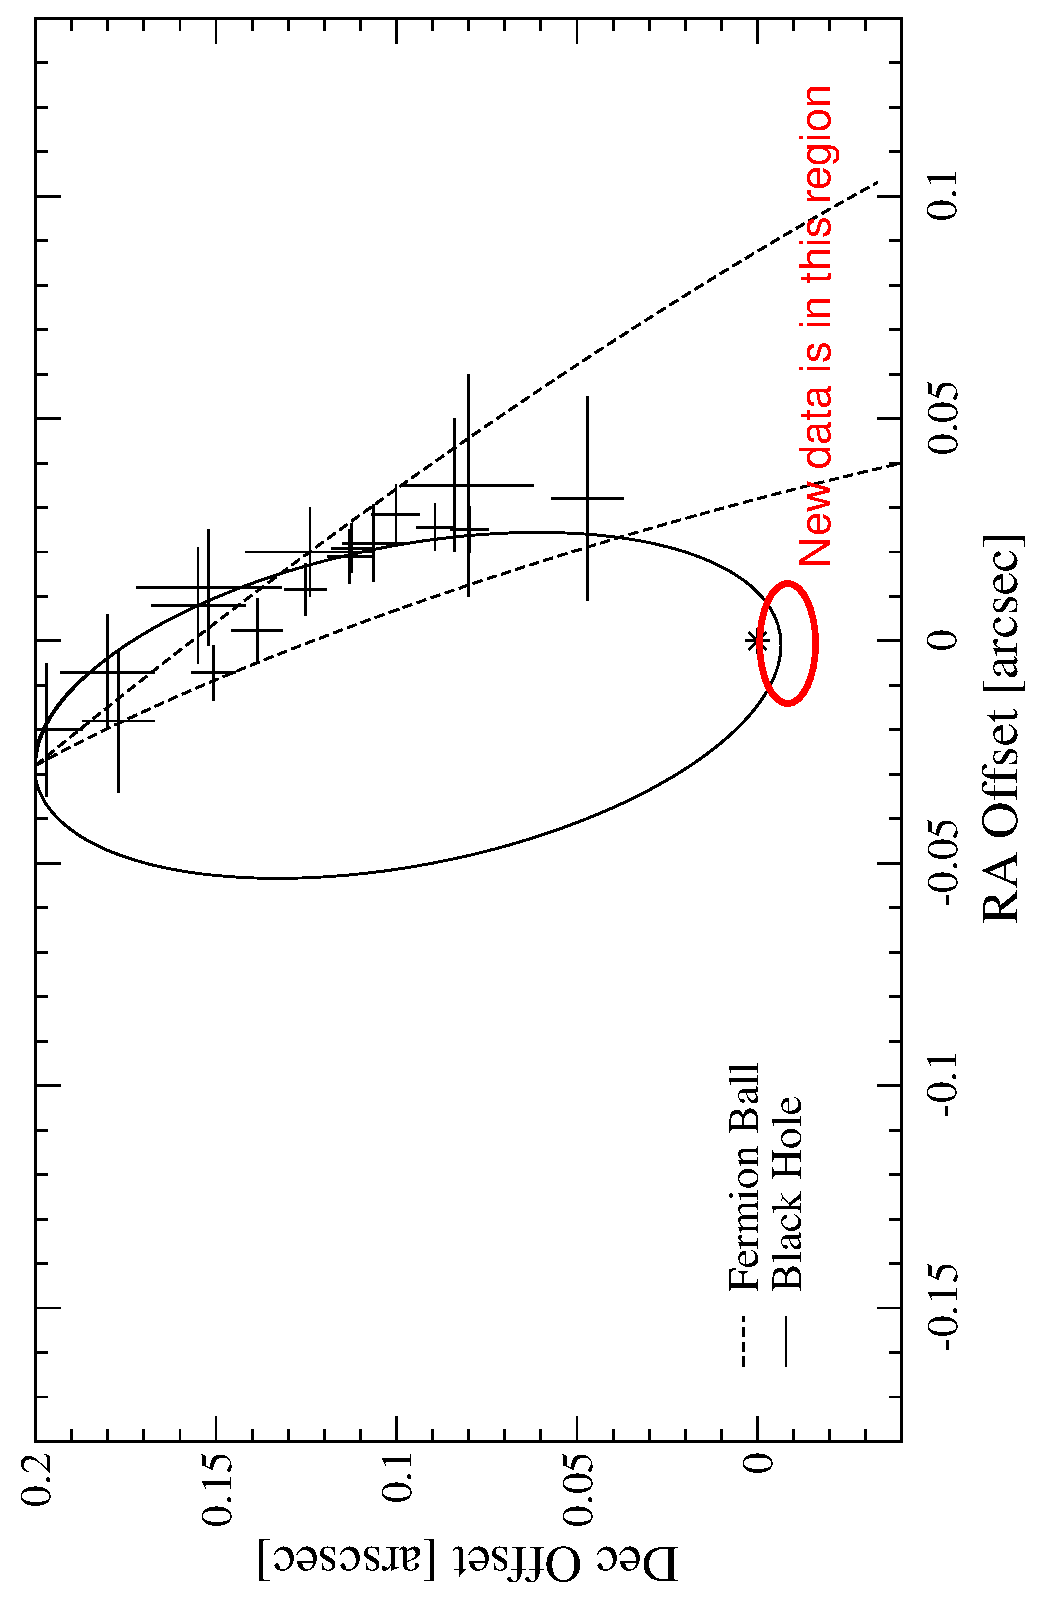
\includegraphics[angle=-90,width=0.9\textwidth]{eps/killer.eps}
	\end{center}
\end{figure}

It is clear that a black hole scenario can account for this new data (albeit with a higher than desired $\chi^2$ value using only
pre-2002 data), but that even the extremal motions for a fermion ball scenario cannot; showing that the fermion ball scenario does
not apply to the centre of our galaxy, and furthering the evidence for a black hole at the centre of the Milky Way.
\clearpage
